Els fotons creats en el plàstic centellejador són detectats pels fotosensors. La col·laboració TRITIUM està investigant dos tipus de fotosensors amb diferents propietats físiques, els tubs fotomultiplicadors (PMTs) i les matrius de fotomultiplicadors de silici (SiPMs), mostrats a la Figura \ref{fig:Fotosensors}. Tots dos utilitzen l'efecte fotoelèctric per transformar els fotons detectats en electrons. El PMT col·lecta i multiplica aquests fotons a través d'una cadena de dinodes mentre que la matriu de SiPMs ho fa en l'interior de fotodiodes d'allau operant en mode Geiger i en paral·lel.

\begin{figure}[htpb]
\centering
    \begin{subfigure}[b]{0.4\textwidth}
    \centering
    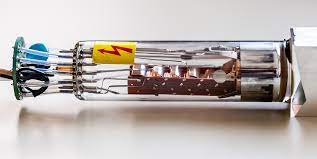
\includegraphics[width=\textwidth]{12Summary/3DesignPrinciples/32Tritium_detector/PMT.jpeg}  
    \caption{\label{subfig:PMT}}
    \end{subfigure}
    \hfill
    \begin{subfigure}[b]{0.4\textwidth}
    \centering
    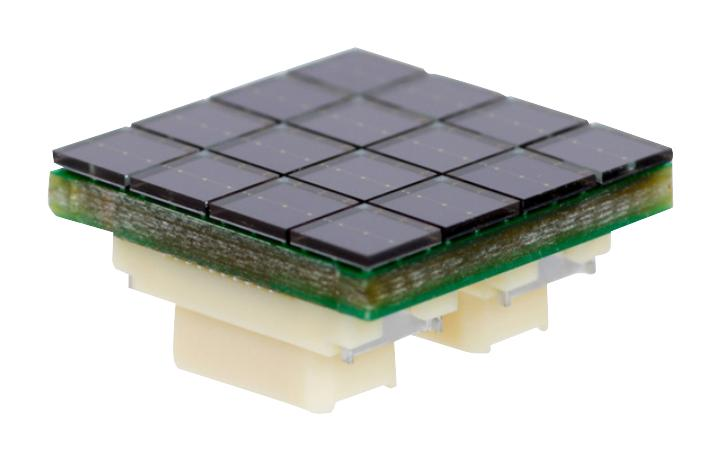
\includegraphics[width=\textwidth]{12Summary/3DesignPrinciples/32Tritium_detector/SiPM_Matrix.jpg}  
    \caption{\label{subfig:SiPM}}
    \end{subfigure}
 \caption{a) Tub fotomultiplicador. b) Matriu de fotomultiplicadors de silici.}
 \label{fig:Fotosensors}
\end{figure}

Els dos fotosensors posseeixen una àrea activa optimitzada per a la detecció de fotons, normalment en l'espectre visible. La probabilitat que el PMT i el SiPM produeixen un senyal com a resposta a la detecció de fotons ve determinada per l'eficiència quàntica i l'eficiència de fotodetecció, respectivament, els espectres dels quals es mostren a la Figura \ref{fig:EficienciaFotosensors} en funció de la longitud d'ona. 
\begin{figure}[htpb]
\centering
    \begin{subfigure}[b]{0.55\textwidth}
    \centering
    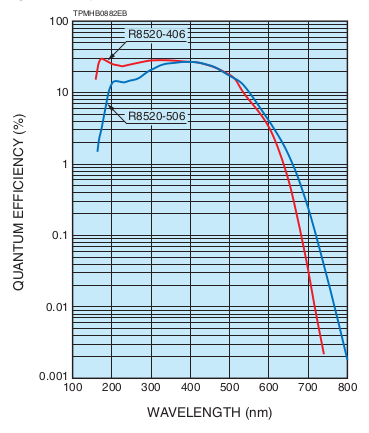
\includegraphics[width=\textwidth]{12Summary/3DesignPrinciples/32Tritium_detector/QuantumEfficiencyPMT.png}  
    \caption{\label{subfig:QEPMT}}
    \end{subfigure}
    \hfill
    \begin{subfigure}[b]{0.55\textwidth}
    \centering
    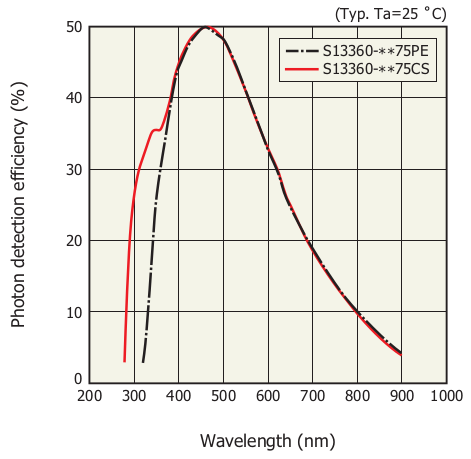
\includegraphics[width=\textwidth]{12Summary/3DesignPrinciples/32Tritium_detector/SiPMPDE.png}  
    \caption{\label{subfig:PDESiPM}}
    \end{subfigure}
 \caption{a) Eficiència quàntica del PMT model R8520-406 de Hamamatsu Photonics \cite{DataSheetPMTs}. b) Eficiència de fotodetecció del fotomultiplicador de silici model S13360-6075 de Hamamatsu Photonics \cite{DataSheetHammamatsu_1_SiPM_1375}.}
 \label{fig:EficienciaFotosensors}
\end{figure}
És important escollir el fotosensor adequat per tal que l'espectre d'emissió del centellejador, Figura \ref{fig:EspectreEmisioPlasticsTRITIUM}, se superpose tant com siga possible amb l'eficiència de detecció del fotosensor, Figura \ref{fig:EficienciaFotosensors}, ja que l'eficiència del detector resultant dependrà del producte de tots dos. Finalment els fotosensors emeten un senyal elèctric que porta informació de l'esdeveniment, el qual és amplificat per a poder ser mesurat i analitzat. Aquest senyal és proporcional al nombre de fotons detectats i, per tant, a l'energia depositada al centellejador per la partícula ionitzant. A partir de cert valor d'energia es perd la linealitat i es produeix allò que s'anomena saturació. Entre les principals diferències entre aquests dos fotosensors trobem que el SiPM no necessita alt voltatge per funcionar (típicament inferior a $70~\volt$), té una major eficiència de detecció i és més robust mentre que el PMT presenta un soroll electrònic més baix. A més, les propietats dels SiPMs varien fortament en funció de la temperatura.

La col·laboració TRITIUM ha realitzat una caracterització detallada dels SiPMs obtenint, amb gran precisió, resultats que estàn d'acord amb els esperats segons el fabricant. A més, s'ha posat a prova amb èxit un protocol per mantenir estable el guany dels SiPMs quan es produeixen variacions de la temperatura. Finalment, entre aquests dos fotosensors emprats, s'escollirà aquell per a qui s'obtinguen millors resultats per a la detecció del triti.